\documentclass[12pt,a4paper]{article}


\usepackage{macros}

\begin{document}\thispagestyle{empty}

\centerline{\Large \bf Homework 4: Due at class on April 1}


 \vspace{.5cm}
 \noindent \textbf{1}. Let $\iota:S^2 \hookrightarrow \bR^3$ be the inclusion of the 2-sphere with unit radius.  Let $g:ds^2=\sum_{i=0}^2dx^i\otimes dx^i$ be the standard metric of $\bR^3$. Find the induced metric $\iota^* g$ on $S^2$ in terms of the polar coordinate of $\bR^3$.
\begin{align}
x^0&=r\sin\theta \cos\phi\cr
x^1&=r\sin\theta \sin\phi\cr
x^2&=r\cos\theta\nonumber
\end{align}
Given this metric, find geodesics on $S^2$ and compute its Riemann, Ricci and scalar curvature.

 Do parallel transport of a vector along a triangle $\Delta$PQR on a unit sphere (Figure 1) with respect to the Levi-Civita connection of the metric and find the angle difference when it comes back.  Compare it with the area of the triangle (see Homework 1).


 \begin{figure}[h]\centering
  \includegraphics[width=5cm]{triangle}
 \caption{A triangle on a 2-sphere}
 \end{figure}

\vspace{.5cm}
\noindent  \textbf{2}. Let $ds^2=-dt^2+dx^2+dy^2$ be the Minkowski metric on $\bR^{1,2}$ and $-t^2+x^2+y^2=-1$ for $t>0$ be the space-like surface (hyperboloid $\mathbf{S}$). (See Figure 1.) Find the induced metric on the hyperboloid $\mathbf{S}$ in terms of the polar coordinate
\begin{align}
t&=r \cosh \rho  \cr
x&=r\sinh\rho\cos\phi\cr
y&=r\sinh\rho \sin\phi\nonumber
\end{align}
Given this metric, find geodesics on $\mathbf{S}$ and compute its Riemann, Ricci and scalar curvature.




\vspace{.5cm}
\noindent  \textbf{3}. Let us consider the unit disk $\mathbf{D}$ on the x-y plane. Let $\pi(P)$ be the intersection point of the unit disk and the line between the  point $(0,0,-1)$ and $P\in \mathbf{S}$. By assigning $\pi(P)$ to $P$, there is one-to-one map from the unit disk $D$ and the hyperboloid $\mathbf{S}$.
Show that the map $\pi^{-1}:\mathbf{D}\to \mathbf{S}$ is determined by
$$
(u,v) \mapsto \left(\frac{2u}{1-u^2-v^2},\frac{2v}{1-u^2-v^2},\frac{1+u^2+v^2}{1-u^2-v^2} \right)~.
$$
Find the metric on the unit disk pull-backed by this map. The unit disk $\mathbf{D}$ with this induced metric is called the Poincar\'e disk.

The red curve on the hyperboloid is an intersection with a plane (pink in Figure 2,3) that goes through the origin. We put a disk (called Klein's disk) on the bottom of the hyperboloid, which allows us to get the corresponding straight line (green) on Klein's disk. This curve is mapped by $\pi:\mathbf{S}\to \mathbf{D}$ to an (red) arc in the Poincare disk. If the green line is represented by $x=a$ (Figure 4), find the equation for the red curve.

Find geodesics on $\mathbf{D}$ and compute its Riemann, Ricci and scalar curvature.

%
% \vspace{.5cm}
% \noindent 6. We consider the unite 2-sphere $S^2\subset \bR^3$ with metric induced from $\bR^3$ as in problem 2. Let us define a smooth map $f:S^2\to \bR$ by $f(x^0,x^1,x^2)=x^2$. Then, explicitly write the gradient vector of $f$ and its flow $\varphi_t$.






\begin{figure}[h]
  \begin{minipage}[b]{8cm}\centering
 \includegraphics[width=8cm]{hyperboloid}
\caption{Hyperboloid and Poincare disk}
\end{minipage}
  \begin{minipage}[b]{8cm}\centering
 \includegraphics[width=6.5cm]{hyperboloid2}
 \caption{Hyperboloid and Poincare disk}
\end{minipage}
\end{figure}

\begin{figure}[h]\centering
 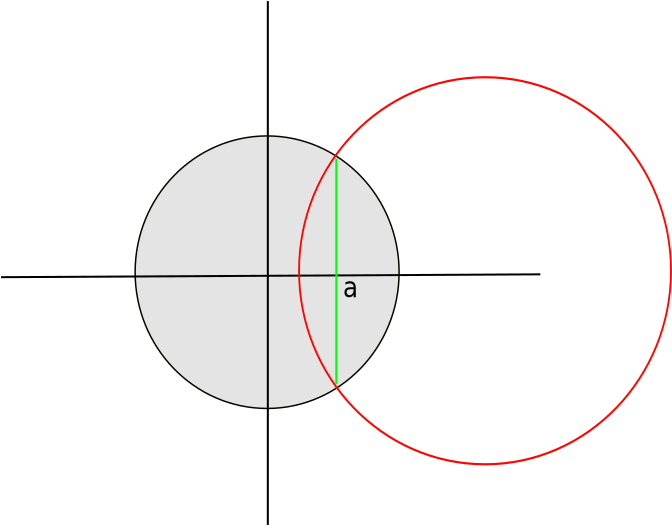
\includegraphics[width=5cm]{disk}
\caption{Poincare disk}
\end{figure}




\end{document}
